% Plantilla para documentos LaTeX para enunciados
% Por Pedro Pablo Aste Kompen - ppaste@uc.cl
% Licencia Creative Commons BY-NC-SA 3.0
% http://creativecommons.org/licenses/by-nc-sa/3.0/

\documentclass[12pt]{article}

% Margen de 1 pulgada por lado
\usepackage{fullpage}
% Incluye gráficas
\usepackage{graphicx}
% Packages para matemáticas, por la American Mathematical Society
\usepackage{amssymb}
\usepackage{amsmath}
% Desactivar hyphenation
\usepackage[none]{hyphenat}
% Saltar entre párrafos - sin sangrías
\usepackage{parskip}
% Español y UTF-8
\usepackage[spanish]{babel}
\usepackage[utf8]{inputenc}
% Links en el documento
\usepackage{hyperref}
\usepackage{fancyhdr}
\setlength{\headheight}{15.2pt}
\setlength{\headsep}{5pt}
\pagestyle{fancy}

\newcommand{\N}{\mathbb{N}}
\newcommand{\Exp}[1]{\mathcal{E}_{#1}}
\newcommand{\List}[1]{\mathcal{L}_{#1}}
\newcommand{\EN}{\Exp{\N}}
\newcommand{\LN}{\List{\N}}

\newcommand{\comment}[1]{}
\newcommand{\lb}{\\~\\}
\newcommand{\eop}{_{\square}}
\newcommand{\hsig}{\hat{\sigma}}
\newcommand{\ra}{\rightarrow}
\newcommand{\lra}{\leftrightarrow}

% Cambiar por nombre completo + número de alumno
\newcommand{\alumno}{Matias Araos, Vicente Rivas, Victor Ruiz - Grupo 15}
\rhead{Entrega 2 - \alumno}

\begin{document}
\thispagestyle{empty}
% Membrete
% PUC-ING-DCC-IIC1103
\begin{minipage}{2.3cm}

\includegraphics[width=2cm]{img/logo.pdf}
\vspace{0.5cm} % Altura de la corona del logo, así el texto queda alineado verticalmente con el círculo del logo.
\end{minipage}
\begin{minipage}{\linewidth}
\textsc{\raggedright \footnotesize
Pontificia Universidad Católica de Chile \\
Departamento de Ciencia de la Computación \\
IIC2413 - Bases de Datos \\}
\end{minipage}


% Titulo
\begin{center}
\vspace{0.5cm}
{\huge\bf Entrega 2}\\
\vspace{0.2cm}
\today\\
\vspace{0.2cm}
\footnotesize{2º semestre 2024 - Profesores Eduardo Bustos  - Christian Alvarez}\\
\vspace{0.2cm}
\footnotesize{\alumno}
\rule{\textwidth}{0.05mm}
\end{center}



\section*{Diagrama E/R}
\begin{center}
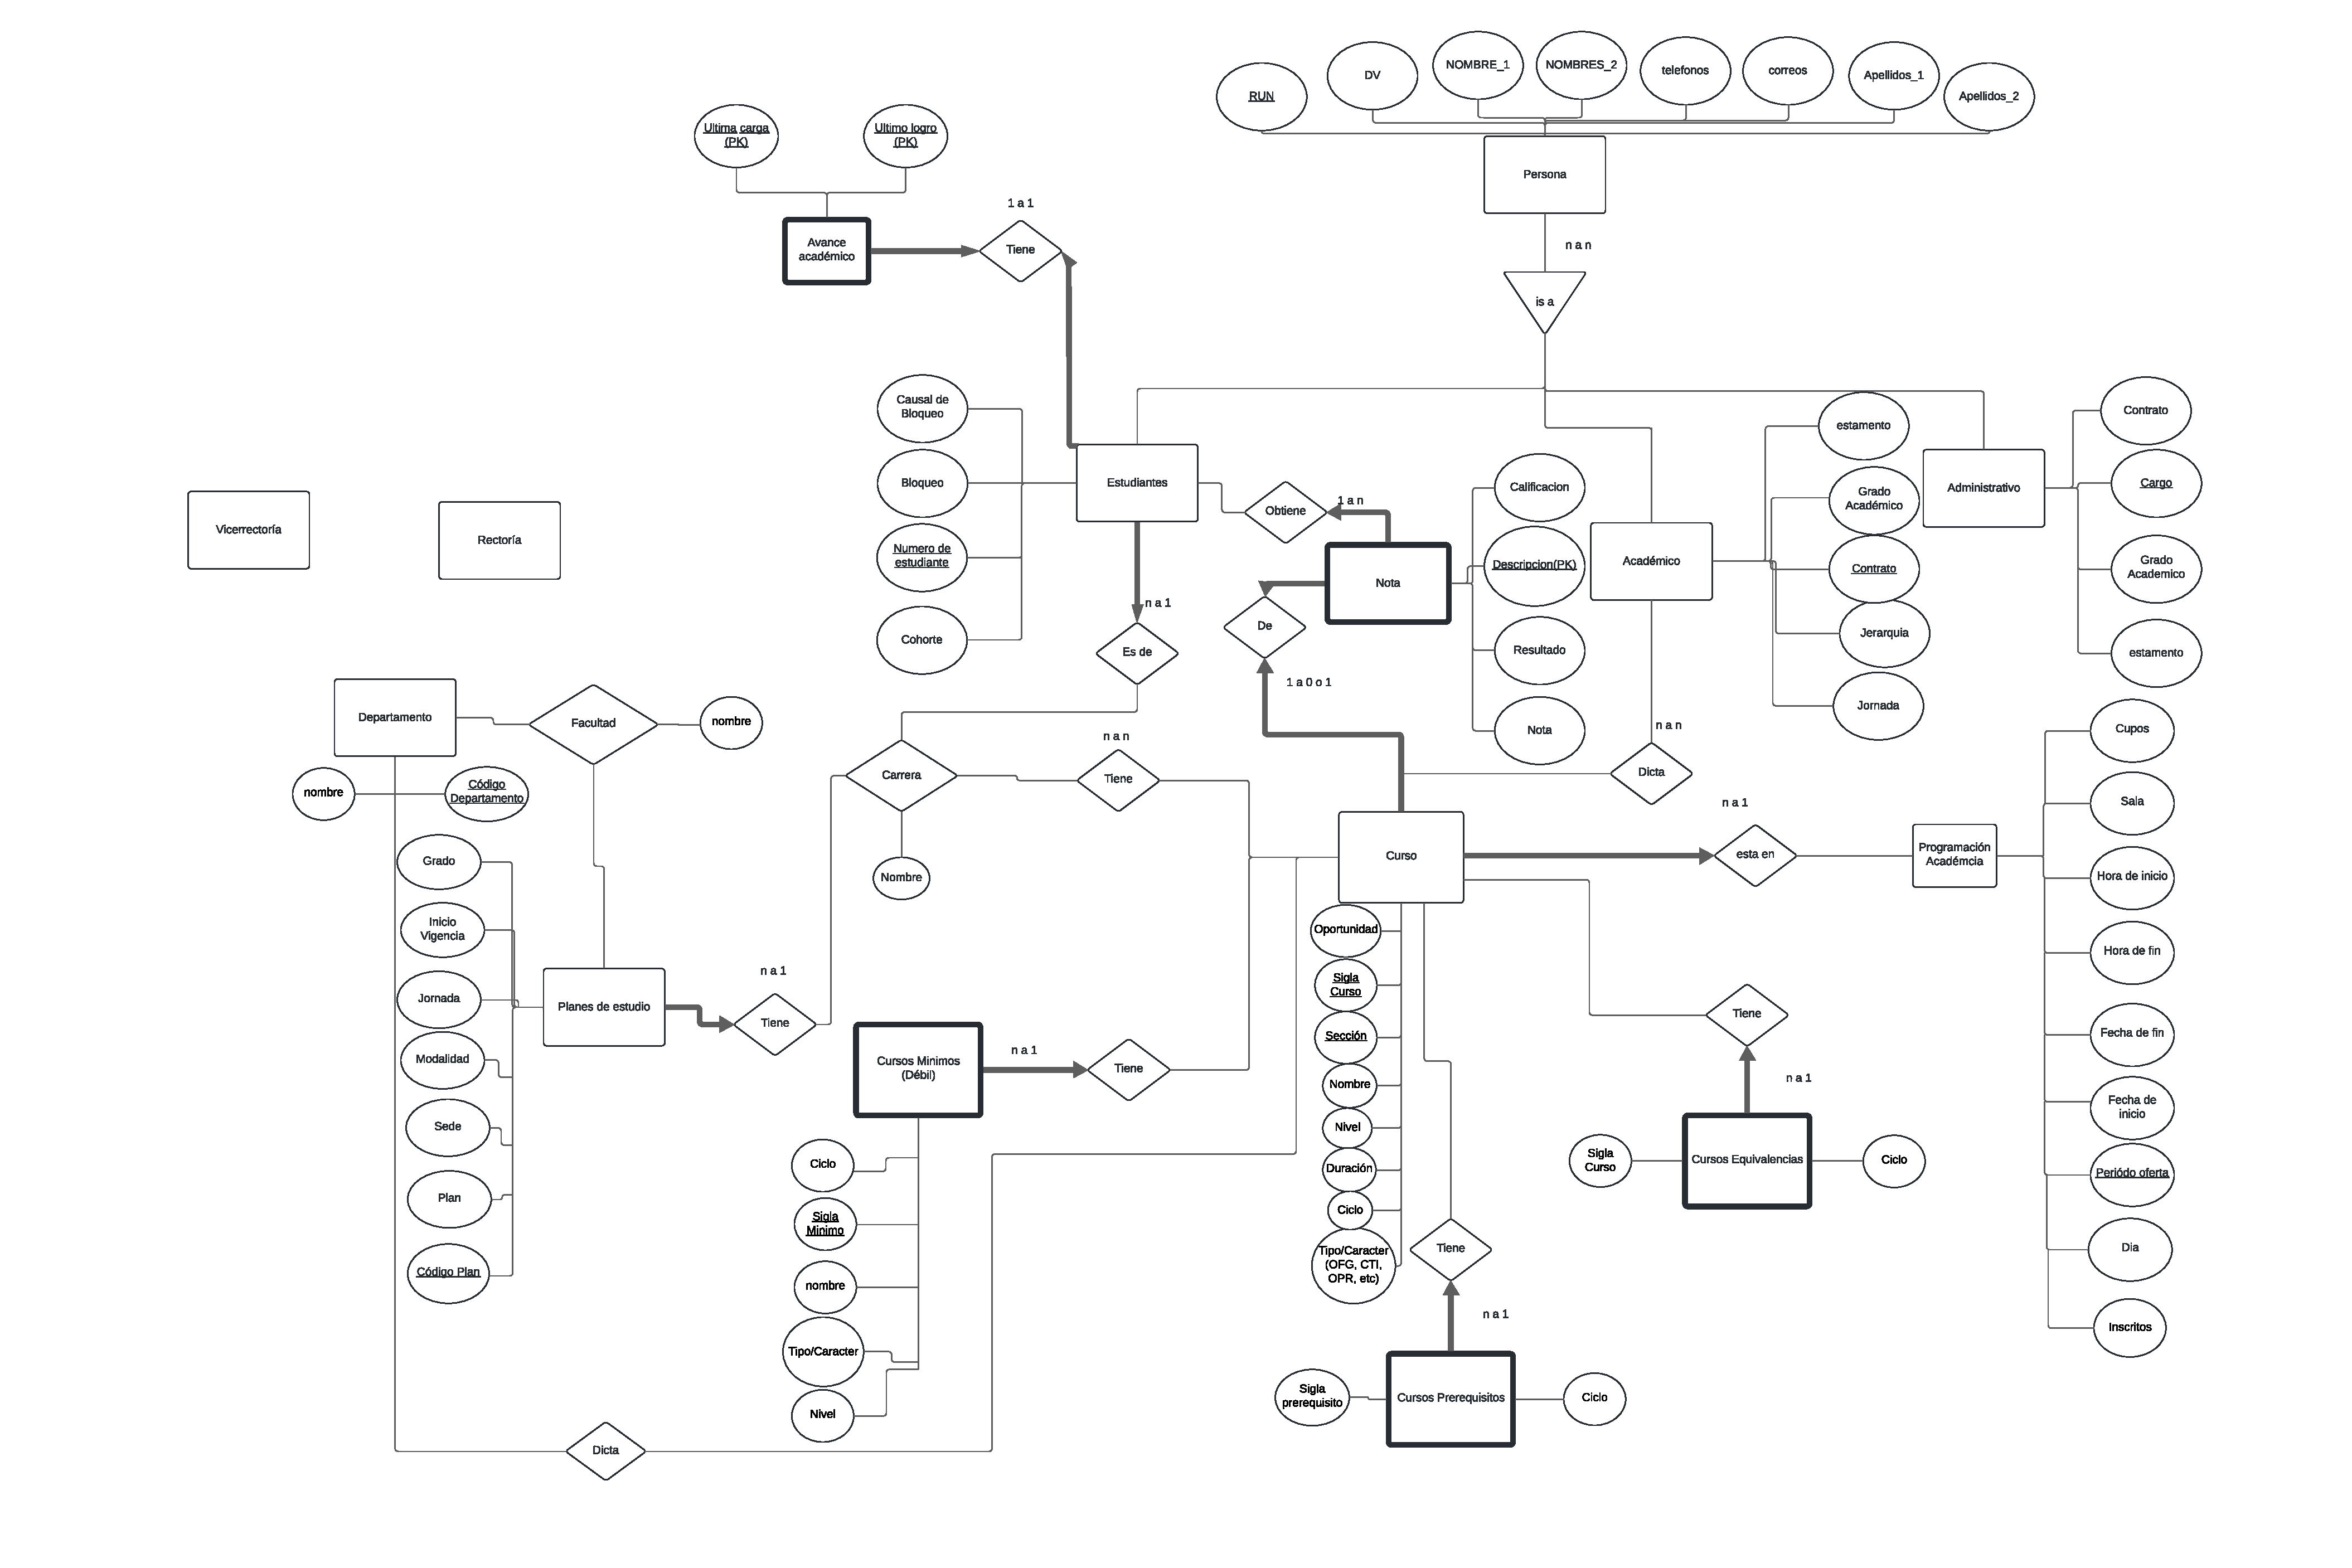
\includegraphics[width=1.1\textwidth]{img/Diagrama_er_1.pdf}
\end{center}
\section*{Entidades Débiles}
\subsection*{Historial Académico}
Es débil porque no puede identificarse de manera única sin asociarse con la entidad 'Estudiante'. 
Su existencia depende directamente de la existencia de un estudiante particular, lo cual se indica por la relación 'Tiene' 
que conecta estas dos entidades. Además, necesita de la entidad 'Oferta académica' 
para poder existir, dado que al asociarse con esta se puede actualizar la última carga. Del mismo modo, sus llaves dependen del Estudiante, lo cual es un requisito fundamental para estar definido como entidad débil 
(Que las llaves de esta entidad débil dependan de otra). 

\subsection*{Nota}
Es una entidad débil porque requiere la existencia de 'Estudiante' y 'Curso' 
para tener sentido y ser identificable. La relación 'De' entre 'Nota' y "Curso", y 'Obtiene' entre 'Nota' y 'Estudiante', 
subraya que una nota no puede existir sin que un estudiante esté inscrito en un curso específico y haya recibido una calificación. 

\subsection*{Prerrequisito}
La entidad 'Prerrequisito' es débil porque no puede existir de manera independiente. 
Su existencia depende directamente de la entidad 'Curso'. Esto se evidencia por la relación 'Tiene' entre 'Curso' y 'Prerrequisito'. 
Un prerrequisito es un curso que debe completarse antes de poder inscribirse en otro curso. Por lo tanto, debe asociado a 
un curso específico. Las llaves primarias de 'Prerrequisito', es decir, Ciclo y Curso restricción, que forman una llave compuesta, no son independientes; 
necesitan estar relacionadas con la llave de 'Curso' (Sigla Curso y Sección), que también forman una llave compuesta 
para poder ser identificada de manera única.  

\newpage
\section*{Llaves Primarias y Parciales}
%subrayamos las llaves primarias
\subsection*{Persona(\underline{RUT})}
Es la llave primaria, pues es un identificador único para cada persona.  
\subsection*{Estudiante(\underline{Número de estudiante})}
Es la llave primaria, pues también identifica de manera única a cada estudiante. Si un Estudiante ingresa a otro plan, de todos modos, se tiene al RUN como carácter diferenciador. 
\subsection*{Historial Académico(\underline{Última Carga}, \underline{Último Logro})}
En conjunto forman una llave parcial que permite, que con ayuda de una llave externa (Estudiante.Número de estudiante), se pueda identificar de manera única a cada historial académico.
\subsection*{Nota(\underline{Descripción})}
Es una llave parcial, ya que no es suficiente para identificar de manera única a una nota, sin embargo
es uno de los elementos que no perimenten valores nulos y siempre da información relevante que en conjunto con llaves externas (Curso.Sigla Curso, Curso.Sección, Estudiante.Número de estudiante) permite identificar de manera única a cada nota.
\subsection*{Carrera(\underline{Nombre Carrera})}
Es la llave primaria, ya que por sí sola permite identificar y distinguir a cada carrera individualmente.
\subsection*{Planes de Estudio(\underline{Código Plan})}
Es la llave primaria, ya que por sí sola permite identificar y distinguir a cada plan de estudio individualmente.
\subsection*{Oferta Académica(\underline{Periodo Oferta})}
Es la llave primaria, ya que por sí sola permite identificar y distinguir a cada oferta académica individualmente.
\vspace*{0.5cm}
\section*{Llaves Compuestas}
\subsection*{Prerrequisito(\underline{Curso.Sigla Curso}, \underline{Curso.Sección}, \underline{Ciclo}, \underline{Curso Restricción})}
Es una llave compuesta, pues requiere tanto de las llaves de Curso para conocer e identificar claramente 
cuáles son los cursos que tienen cursos prerrequisitos, así como también el Ciclo y Curso restricción para dar cuenta del periodo académico y de los cursos restringidos por el prerrequisito. 
\subsection*{Nota(\underline{Curso.Sigla Curso}, \underline{Curso.Sección}, \underline{Descripción}, 
\\ \underline{Estudiante.Número de estudiante})}
Es una llave compuesta, dado que requiere de esas llaves para lograr dar una identificación clara y única de la nota buscada, según el curso al que pertenece y el propio resultado de la nota (a través de la llave Descripción). 
\subsection*{Historial Académico(\underline{Estudiante.Número de estudiante}, \underline{Curso.Sigla Curso}, \underline{Curso.Sección}, \underline{Última Carga}, \underline{Último Logro})}
Es una llave compuesta, pues sirven para identificar de manera única cada curso que el Estudiante ha tomado a lo largo de su carrera. 
\subsection*{Curso(\underline{Sigla Curso}, \underline{Sección})}
Es una llave compuesta ya que, si bien la sigla del curso permite identificar y distinguir por si sola a cada curso, usar a las Secciones como parte de la Llave nos permite una mayor identificación para así diferenciar entre las distintas secciones de cada asignatura.  
\newpage
\section*{Cardinalidad}
\subsection*{Persona Is A Estudiante / Académico / Administrativo: (n, n)}
Una Persona puede ser un estudiante, académico, administrativo, o cualquier combinación de los tres roles, por lo tanto, una persona puede tener más de un rol, como administrativo, 
y a su vez, hay otros n administrativos que también son personas. 
\subsection*{Estudiante Tiene Historial Académico: (1, 1)}
Un estudiante tiene un solo historial académico, y cada historial está asociado únicamente a un solo estudiante. 
\subsection*{Estudiante Obtiene Nota (Entidad Débil): (1, n)}
Un Estudiante puede tener múltiples Notas, pero cada nota va a pertenecer únicamente a un solo Estudiante. 
\subsection*{Estudiante Es De Carrera: (n, 1)}
Un estudiante puede pertenecer a una carrera solo, y una carrera puede tener muchos estudiantes inscritos.  
\subsection*{Carrera Tiene Planes de Estudio: (1, n)}
Cada Carrera puede tener varios planes de estudio, pero un plan de estudio se asocia únicamente a una carrera.  
\subsection*{Carrera Tiene Curso: (n, n)}
Una carrera puede tener varios cursos, y un curso puede a su vez pertenecer a varias carreras. 
\subsection*{Nota De Curso: (1, 1)}
Cada Nota va a corresponder a un solo curso, pero cada curso tiene 1 nota.
\subsection*{Académico Dicta Curso: (n, n)}
Un Académico puede dictar varios cursos, y un curso puede ser dictado por varios Académicos. 
\subsection*{Curso Tiene Prerrequisito (Entidad Débil): (1, 1)}
Un curso puede tener 1 prerrequisito, y esos cursos prerrequisito están relacionadas a un Curso.  
\subsection*{Curso Esta En Oferta Académica: (n, n)}
Un curso puede estar en varias ofertas académicas, y en una oferta académica hay varios cursos.
\section*{Jerarquías de Clase}
\subsection*{Persona \textgreater \; Estudiante // Académico // Administrativo}
Persona es una superclase, cuyos atributos (RUN, DV, Nombres, Correo, Teléfono) son compartidos por todas las personas, a todos los miembros de la comunidad que derivan de Persona, en este caso: Estudiante, Académico y Administrativo, que poseen atributos propios que no comparten necesariamente con los otros. 
\section*{Esquema Relacional}
\textit{Persona}(\underline{RUT}: int, \underline{DV}: int, Nombres: string, Apellido\_Paterno: string, Apellido\_Materno: string, Nombre\_Completo: string, Mail\_Personal: string, Mail\_Institucional: string, Teléfono: string) \\\\
\textit{Estudiante}(\underline{Persona.RUT}: int, \underline{Persona.DV}: int, \underline{Número\_de\_Estudiante}: int, Carrera: string, Cohorte: string, Estado: string, Bloqueo: bool) \\\\
\textit{Académico}(\underline{Persona.RUT}: int, \underline{Persona.DV}: int, Contrato: string, Jerarquía: string, Jornada: string, Grado\_Académico: string) \\\\
\textit{Administrativo}(\underline{Persona.RUT}: int, \underline{Persona.DV}: int, Cargo: string, Grado\_Académico: string) \\\\
\textit{Curso}(\underline{Sigla\_Curso}: string, \underline{Sección}: int, Nombre: string, Nivel: string, Tipo/Carácter (OFG, CTI, OPR, etc.): string, Ciclo: int, Departamento.Código\_Departamento: string) \\\\
\textit{Cursos\_Equivalencias}(\underline{Curso.Sigla\_Curso}: string, \underline{Curso.Sección}: int, Sigla\_Equivalente: string, Ciclo: int) \\\\
\textit{Cursos\_Prerequisitos}(\underline{Curso.Sigla\_Curso}: string, \underline{Curso.Sección}: int, Sigla\_Prerequisito: string, Ciclo: int) \\\\
\textit{Cursos\_Minimos}(\underline{Curso.Sigla\_Curso}: string, \underline{Curso.Sección}: int, Curso\_Minimo: string, Ciclo: int) \\\\
\textit{Planes\_Estudio}(\underline{Código\_Plan}: string, Nombre: string, Facultad: string, Nivel: string, Modalidad: string, Fecha\_Inicio: string) \\\\
\textit{Programacion\_Academica}(\underline{Curso.Sigla\_Curso}: string, \underline{Curso.Sección}: int, Periodo: string, Sala: string, Horario: string, Vacantes: int) \\\\
\textit{Departamento}(\underline{Código\_Departamento}: string, Nombre: string, Facultad: string) \\\\
\textit{Nota}(\underline{Curso.Sigla\_Curso}: string, \underline{Curso.Sección}: int, \underline{Estudiante.Número\_de\_Estudiante}: int, Ciclo: int, Nota: float, Descripción: string, Calificación: string, Resultado: string) \\\\
\textit{Avance\_Academico}(\underline{Estudiante.Número\_de\_Estudiante}: int, \underline{Curso.Sigla\_Curso}: string, \underline{Curso.Sección}: int, Última\_Carga: string, Último\_Logro: string)

\subsection*{Restriciones de Integridad y Dominios}
% Aca avismaos con un diclaimer que si en el dominio exite nulo entonces adimete nulo si no, se asueme que no admite nulo, lo ponemos en mayuscula para que se note
% Ponemos en mayuscula el aviso:
\textbf{Nota:} Si en el dominio existe nulo entonces admite nulo, si no, se asume que no admite nulo.\\\\
\textit{Nota.Calificación} $\in$ \{SO, MB, B, SU, I, M, MM, NP, EX, A, R, nulo\}\\\\\
\textit{Prerrequisito.Ciclo} $\in$ \{B, L\}\\\\
\textit{Estudiante.Bloqueo} $\in$ \{S, N\}\\\\
\textit{Académico.Jornada} $\in$ \{Completa, Diurna, Vespertina\}\\\\
\textit{Oferta Académica.Módulo Horario} $\in$ \{1, 2, 3, 4, 5, 6, 7, 8, 9\}\\\\
\textit{Persona.DV} $\in$ \{0, 1, 2, 3, 4, 5, 6, 7, 8, 9, K\}\\\\
% Curso.Nivel tiene dos dominios, 1...10 o B, L, lo agregamos con una disyunción
\textit{Curso.Nivel} $\in$ \{1, 2, 3, 4, 5, 6, 7, 8, 9, 10\} $\cup$ \{B, L\}\\\\
\textit{Nota.Descripción} $\in$ \{Sobresaliente, Muy Bueno, Bueno, Suficiente, Insuficiente, Malo, Muy Malo, Nota Pendiente, Eximido, Aprobado, Reprobado, curso vigente\}\\\\
\textit{Nota.Nota} $\in$ \{1.0 - 1.9, 2.0 - 2.9, 3.0 - 3.9, 4.0 - 4.9, 5.0 - 5.9, 6.0 - 6.5, 6.6 - 7.0, nulo\}\\\\
\textit{Nota.Resultado} $\in$ \{Aprobatorio, Reprobatorio, Curso incompleto, Curso Vigente en el período académico\}\\\\
\textit{Historial Académico.Último Logro} $\in$ \{Ingreso, 1...10, Licenciatura\}\\\\
\textit{Historial Académico.Última Carga} $\in$ \{año-semestre\}\\\\
\textit{Estudiante.Cohorte} $\in$ \{año-semestre\}\\\\
\textit{Oferta Académica.Periodo Oferta} $\in$ \{año-semestre\} \newpage
\section*{Tablas de Relaciones}
% Crear tabla: Relaciones muchos a muchos (n:n) y relaciones con atributos propios.
% No crear tabla: Relaciones uno a muchos (1:n) y uno a uno (1:1), a menos que haya una razón específica para hacerlo.

% creamos las tablas de solos los que son n a n
% Las tablas a partir de relaciones a crear serían: Persona_Rol (con sus 3 respectivos roles: Estudiante, Académico, Administrativo), Curso_Carrera, Curso_Académico y Curso_Oferta Académica.

\textit{Persona\_Rol}(\underline{Persona.RUT}: int, \underline{Estudiante.Número de estudiante}: int, \underline{Académico.Persona.RUT}: int, \underline{Administrativo.Persona.RUT}: int)\\\\
\textit{Curso\_Carrera}(\underline{Curso.Sigla Curso}: string, \underline{Curso.Sección}: int, \underline{Carrera.Nombre Carrera}: string)\\\\
\textit{Curso\_Académico}(\underline{Curso.Sigla Curso}: string, \underline{Curso.Sección}: int, \underline{Académico.Persona.RUT}: int)\\\\
\textit{Curso\_Oferta\_Académica}(\underline{Curso.Sigla Curso}: string, \underline{Curso.Sección}: int, \underline{Oferta Académica.Periodo Oferta}: string)

\section*{Temas que resuelve el Esquema}
\subsection*{Fidelidad}
El esquema refleja con bastante claridad y precisión la estructura universitaria de nuestro caso, considerando variables como cuando un Estudiante puede ser un Académico y Administrativo al mismo tiempo, lo cual contribuye bastante a una clara representación de la realidad a través de nuestro modelo y esquema, respetando las reglas de negocio y complementándolas con aquellas de la entrega anterior, caracterizando así a través de sus atributos, a cada entidad de la forma que mejor las pueda representar, es decir, hay un válida relación entre las distintas entidades.  
\subsection*{Redundancia}
Dado que Persona actúa como Superclase para Estudiante, Académico y Administrativo, se evitan grandes problemas de redundancia al no tener que repetir los mismos atributos varias veces, por lo que se ha minimizado la problemática de redundancia. Además, el uso de llaves foráneas es también de gran ayuda a la hora de abordar esto, disminuyendo así la necesidad de duplicar información en varias entidades. Esto se ve reflejado igualmente con el uso de llaves compuestas y parciales, de modo que cada entidad débil pueda acceder a información vital para ellas a través de otras entidades, como es el caso de la entidad 'Nota', que accede a las llaves de la entidad 'Curso'. (Sigla Curso y Sección).
\subsection*{Anomalías}
La poca redundancia existente gracias al uso de llaves compuestas implementadas adecuadamente da lugar a una menor cantidad de anomalías. No existen atributos redundantes, y se siguen las reglas de negocio, además de un variado uso de llaves bien definidas, por lo que no deberían haber mayores problemáticas de anomalías. 
\subsection*{Simplicidad}
Se intenta no complicarse más de la cuenta, y esto se ve en la poca redundancia que existe ya que el esquema maneja entidades bien definidas. 
\subsection*{Buena elección de llaves primarias}
A través de una buena etapa de diseño, fue posible identificar llaves candidatas \textit{natural keys} que luego fueron convertidas a llaves primarias, buscando que fueran únicas y poco redundantes. Por ejemplo, casos como el de la llave primaria de la entidad
'Persona', RUN, es una muy buena elección, ya que esta debiese ser única para cada persona, y dado que esa entidad funciona como una superclase para las demás, es fácilmente utilizable por las entidades Persona, Académico o Administrativo. La misma lógica sigue para las llaves de las entidades 
'Estudiante' y 'Curso', respectivamente: Número de Estudiante y Sigla Curso, junto a Sección, forman llaves particularmente fuertes, permitiendo diferenciar e identificar a cada estudiante, así como los cursos de estos. Además, son llaves generalmente minimalistas, que no incluyen atributos innecesarios que podrían complicar el sistema a futuro, y también son bastante estables, ya que no se alteran mucho con el tiempo; por ejemplo, el RUN debiese ser siempre el mismo.

% Fin del documento
\end{document}
